\documentclass[tikz,border=2pt]{standalone}
\usepackage{amsmath,amssymb}
\usepackage{tikz}
\usetikzlibrary{matrix}

\begin{document}
% The Hessian collects all second-order partial derivatives; for a C^2 function it is
% symmetric and gives the quadratic term of the Taylor expansion.
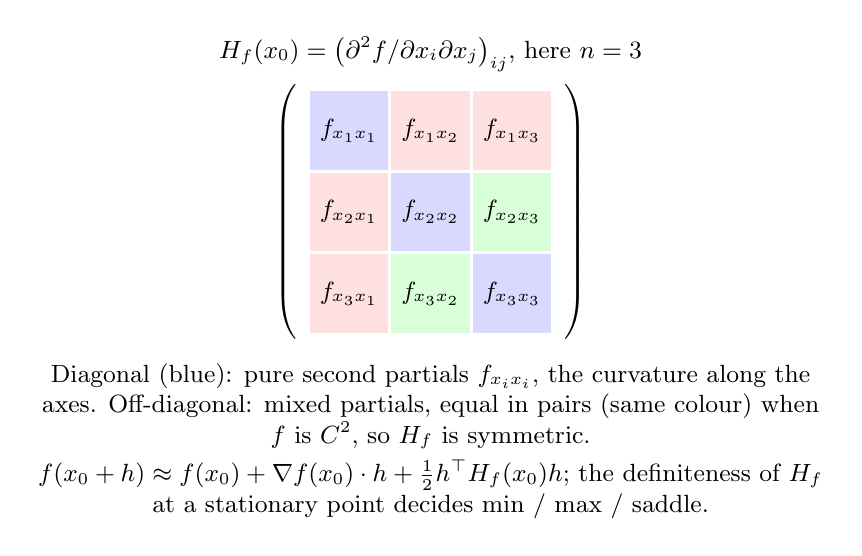
\begin{tikzpicture}[every node/.style={font=\small}]
	\matrix (H) [matrix of math nodes, nodes={minimum size=1.0cm, anchor=center}, left delimiter=(, right delimiter=), column sep=1pt, row sep=1pt] at (0,0) {
		|[fill=blue!15]| f_{x_1x_1} & |[fill=red!12]| f_{x_1x_2} & |[fill=red!12]| f_{x_1x_3} \\
		|[fill=red!12]| f_{x_2x_1} & |[fill=blue!15]| f_{x_2x_2} & |[fill=green!15]| f_{x_2x_3} \\
		|[fill=red!12]| f_{x_3x_1} & |[fill=green!15]| f_{x_3x_2} & |[fill=blue!15]| f_{x_3x_3} \\
	};
	\node[anchor=south] at (H.north) {$H_f(x_0)=\big(\partial^2f/\partial x_i\partial x_j\big)_{ij}$, here $n=3$};
	\node[anchor=north, align=flush center, text width=10cm] at ([yshift=-4pt]H.south) {Diagonal (blue): pure second partials $f_{x_ix_i}$, the curvature along the axes. Off-diagonal: mixed partials, equal in pairs (same colour) when $f$ is $C^2$, so $H_f$ is symmetric.\\[3pt] $f(x_0+h)\approx f(x_0)+\nabla f(x_0)\cdot h+\tfrac12h^{\top}H_f(x_0)h$; the definiteness of $H_f$ at a stationary point decides min / max / saddle.};
\end{tikzpicture}
\end{document}
